\documentclass[tikz]{standalone}

\usepackage[utf8]{inputenc}
\usepackage[T1]{fontenc}
\usepackage{times}

\begin{document}

%    foodmart 0.005\%
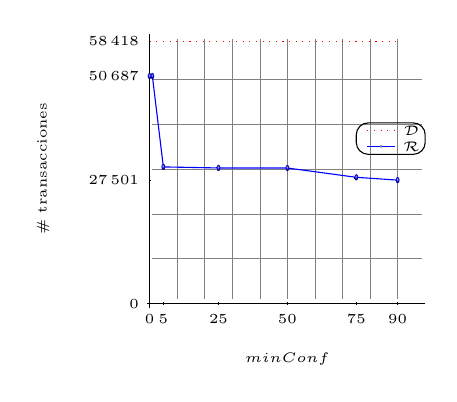
\begin{tikzpicture}[xscale=.35, yscale=.57]
   %ejes
   \draw (-0.1,0) -- (10,0);
   \draw (0,-0.1) -- (0,6);
   \draw[help lines,step=1cm] (0.1,0.1) grid (9.9,5.9);
   %marcas eje X
   \draw (5cm,-35pt) node {\tiny $minConf$};
   \draw (0cm,1pt) -- (0cm,-1pt) node[anchor=north] {\tiny 0};
   \draw (.5cm,1pt) -- (.5cm,-1pt) node[anchor=north] {\tiny 5};
   \draw (2.5cm,1pt) -- (2.5cm,-1pt) node[anchor=north] {\tiny 25};
   \draw (5cm,1pt) -- (5cm,-1pt) node[anchor=north] {\tiny 50};
   \draw (7.5cm,1pt) -- (7.5cm,-1pt) node[anchor=north] {\tiny 75};
   \draw (9cm,1pt) -- (9cm,-1pt) node[anchor=north] {\tiny 90};
   %marcas eje Y
   \draw (-110pt,3 cm) node[rotate=90] {\tiny \# transacciones};
   \draw (1pt,0 cm) -- (-1pt,0 cm) node[anchor=east] {\tiny 0};
   \draw (1pt,2.7501 cm) -- (-1pt,2.7501 cm) node[anchor=east] {\tiny 27\,501};
   \draw (1pt,5.0687 cm) -- (-1pt,5.0687 cm) node[anchor=east] {\tiny 50\,687};
   \draw (1pt,5.8418 cm) -- (-1pt,5.8418 cm) node[anchor=east] {\tiny 58\,418};
   %       \draw (-0.2,-0.5) -- node[right=1pt,fill=white] {\tiny 5\%};
   %líneas
   \draw[color=red,style=dotted] plot coordinates {(0,5.8418) (.1,5.8418) (.5,5.8418) (2.5,5.8418) (5.0,5.8418) (7.5,5.8418) (9.0,5.8418)};
   \draw[color=blue,style=solid] plot[mark=ball] coordinates {(9.0,2.7501) (7.5,2.8125) (5.0,3.0201) (2.5,3.0212) (.5,3.0440) (.1,5.0687) (0,5.0687)};
   %leyenda
   \pgftransformyscale{.35}
   \pgftransformyshift{2cm}
   \draw[rounded corners=1ex] (7.5,7.5) rectangle (10,9.5);
   \draw (9.5,9) node(a) {\tiny$\mathcal{D}$};
   \draw (9.5,8) node(a) {\tiny$\mathcal{R}$};
   \draw[color=red,style=dotted] plot coordinates {(7.9,9) (8.9,9)};
   \draw[color=blue,style=solid] (7.9,8) -- (8.9,8) plot[mark=ball] coordinates {(8.4,8)};
\end{tikzpicture}

\end{document}
